\item An aircraft loops the loop of radius \( R = 500 \text{ m} \) with a constant velocity \( v = 360 \text{ km per hour} \). Find the weight of the flyer of mass \( m = 70 \text{ kg} \) in the lower, upper, and middle points of the loop.
    \begin{center}
        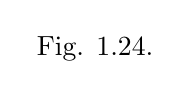
\begin{tikzpicture}
            \node at (0, 0) {Fig. 1.24.};
        \end{tikzpicture}
    \end{center}